\ifdefined\maindoc
% Under the thesis build, main.tex owns the full \graphicspath list. \graphicspath REPLACES
% rather than appends, so this branch deliberately does nothing.
\else
\documentclass[12pt]{report}
\usepackage[a4paper,margin=1in]{geometry}
\usepackage[utf8]{inputenc}
\usepackage[T1]{fontenc}
\usepackage[british]{babel}
\usepackage{amsmath,amssymb,amsthm}
\usepackage{booktabs}
\usepackage{setspace}
\usepackage{graphicx}
\usepackage{enumitem}
\usepackage{placeins}
\usepackage{hyperref}
\usepackage{array}
\usepackage{algorithm}
\usepackage{algpseudocode}
\usepackage[backend=biber,style=ieee,citestyle=numeric-comp,sorting=none]{biblatex}
\addbibresource{../../references.bib}
\setcounter{biburllcpenalty}{7000}
\setcounter{biburlucpenalty}{8000}
\setcounter{biburlnumpenalty}{9000}
\onehalfspacing
\graphicspath{{figures/}}
\newtheorem{theorem}{Theorem}[chapter]
\newtheorem{definition}[theorem]{Definition}
% Standalone-only fallbacks. Numbering: 1 Introduction, 2 Background, 3 this chapter,
% 4 Network Decomposition, 5 Probability, 6 Capacity Flow, 7 Critical Path, 8 Julia package,
% 9 Interface, 10 Integrated Case Study, 11 Conclusions.
\makeatletter
\newlabel{ch:main-intro}{{1}{1}{}{Doc-Start}{}}
\newlabel{ch:lit-review}{{2}{1}{}{Doc-Start}{}}
\newlabel{ch:diamond-module}{{4}{1}{}{Doc-Start}{}}
\newlabel{ch:probability-toolkit}{{5}{1}{}{Doc-Start}{}}
\newlabel{ch:capacity-toolkit}{{6}{1}{}{Doc-Start}{}}
\newlabel{ch:critical-path}{{7}{1}{}{Doc-Start}{}}
\newlabel{ch:julia-package}{{8}{1}{}{Doc-Start}{}}
\newlabel{ch:front-end}{{9}{1}{}{Doc-Start}{}}
\newlabel{ch:integrated-case-study}{{10}{1}{}{Doc-Start}{}}
\newlabel{ch:conclusions}{{11}{1}{}{Doc-Start}{}}
\makeatother
\begin{document}
\title{Complex Processes as Directed Acyclic Graphs}
\fi

\section{Introduction}
\label{sec:model-intro}

The framework rests on a single model of the systems it analyses. This chapter defines that
model and the object built from it, which every later chapter reads. Section~\ref{sec:model-mapping}
describes how a process system is mapped to a directed acyclic graph and discusses the
acyclicity assumption. Section~\ref{sec:model-roles} gives the physical meaning of the node roles.
Section~\ref{sec:model-formal} states the definitions and notation used throughout the
thesis. Section~\ref{sec:model-layers} establishes the layered processing order and the
ancestry closures on which every algorithm in the framework depends.
Section~\ref{sec:model-information} describes the values that an analysis attaches to the
network, the three interpretations of those values, and the three forms in which a value can be
known. Section~\ref{sec:model-input} describes how a model is built from the files in which
real systems are described, and Section~\ref{sec:model-assumptions} states the assumptions
that all later results are conditional on.

\section{From Process to Graph}
\label{sec:model-mapping}

A component is any unit of the system that can carry a value of its own, such as a pump or
a treatment stage. A dependency is the relation in which one component
feeds, supplies or precedes another. The model represents each component as a node and each
dependency as a directed edge. In a goal-oriented process system, one in which a resource moves through the components
towards a delivery point, the relation between
two connected components is already directed. For example, water leaves the intake and arrives
at the pump, and the pump does not supply the intake. Hence the direction of an edge is read off the system.

The model further requires that the directed edges form no cycle. For many of the systems of interest this
holds without further assumption. For example, treatment trains and project schedules move
material or work strictly forward, and a dependency cycle in a schedule would be a planning
error. For other systems, however, acyclicity is
imposed by orienting the network.
A distribution pipe can in principle carry water in either direction, but a network operating
around its design flows has a dominant direction on every pipe, and orienting each edge by that
dominant flow gives a directed acyclic snapshot of the operating regime. The orientation excludes regimes far from the snapshot, such as flow reversal under unusual
demand, recirculation loops and feedback control, and
Section~\ref{sec:model-assumptions} returns to what that exclusion means for the results.
Figure~\ref{fig:model-mapping} shows the mapping on a small treatment process. The process
duplicates its treatment stage, and the duplication appears in the graph as a pair of parallel
routes that later reconverge, which is the structural pattern Section~\ref{sec:model-roles}
names.

\begin{figure}[htbp]
  \centering
  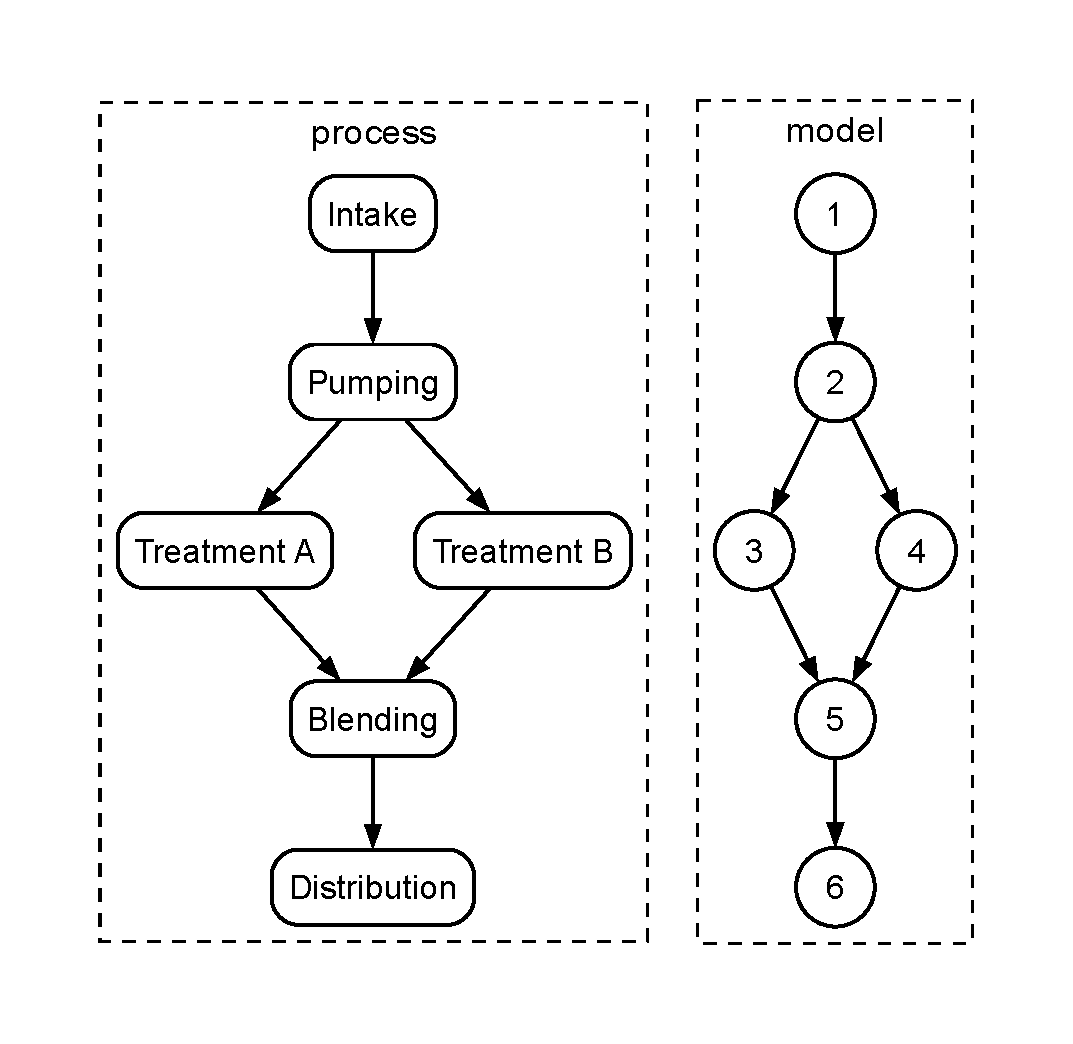
\includegraphics[width=0.78\linewidth]{fig01_mapping/fig01_mapping.pdf}
  \caption{A small treatment process and its model. Components become nodes, dependencies
  become directed edges, and the duplicated treatment stage becomes a pair of parallel routes
  that later reconverge.}
  \label{fig:model-mapping}
\end{figure}

\section{Node Roles}
\label{sec:model-roles}

The position of a node in the network gives it a role, and each role has a physical meaning. A
node with no incoming edge is a source, the point where supply, material or work enters the
system (e.g.\ an intake or the start of a project). Similarly, a node with no
outgoing edge is a sink, where the system delivers (e.g.\ a demand point or a completed
handover). A node that feeds two or more downstream components is a fork. Forks are
how a system distributes and, in particular, how it builds in redundancy, because providing two
routes to the same destination begins with one component supplying two. Finally, a node fed by
two or more components is a join. This is where distributed flows gather and where redundant
routes come back together.

A robust system duplicates its critical routes, and duplicated routes must reconverge at
the destination they protect. A well-designed network therefore contains many
pairs of paths that separate at a fork and meet again at a join while sharing the components
upstream of the fork. Whether that sharing matters depends on the question being asked.
Chapter~\ref{ch:diamond-module} makes the pattern precise, and
Chapter~\ref{ch:probability-toolkit} shows that for the probabilistic interpretation of the model,
ignoring it gives wrong answers. For the present chapter it is enough to note that reconvergence is common in the systems
being modelled. Figure~\ref{fig:model-roles}
shows it on a small network.

\begin{figure}[htbp]
  \centering
  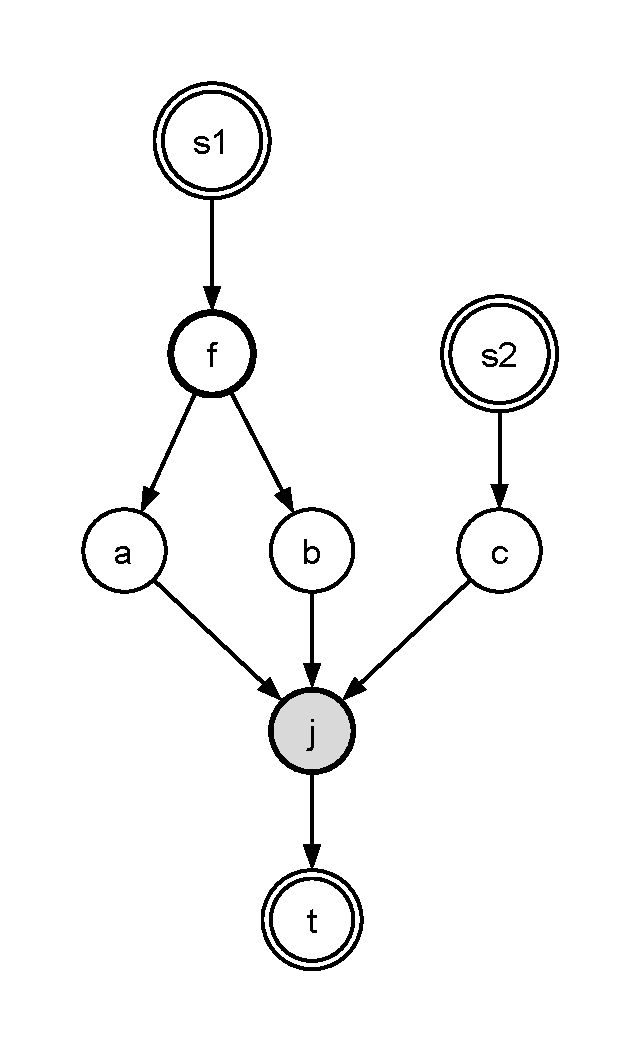
\includegraphics[width=0.5\linewidth]{fig02_roles/fig02_roles.pdf}
  \caption{Node roles on a small network. Double borders mark the source and the sink, the
  bold outline marks the fork, and the shaded node is the join where the redundant pair of
  routes reconverges alongside an independent supply.}
  \label{fig:model-roles}
\end{figure}

\section{Definitions and Notation}
\label{sec:model-formal}

\begin{definition}[Network model]
\label{def:model-network}
A system is modelled as a finite directed acyclic graph $G=(V,E)$ with node set $V$ and edge
set $E \subseteq V \times V$. The sources $S \subseteq V$ are the nodes with no incoming edge
and the sinks $T \subseteq V$ the nodes with no outgoing edge. For a node $v$, $\mathrm{Pa}(v)$
denotes its parents, the nodes with an edge into $v$, and $\mathrm{Ch}(v)$ its children.
\end{definition}

\begin{definition}[Ancestry]
\label{def:model-ancestry}
A node $u$ is an ancestor of $v$ when a directed path leads from $u$ to $v$, and a descendant
when one leads from $v$ to $u$. The sets $\mathrm{anc}(v)$ and $\mathrm{desc}(v)$ collect them.
Throughout the framework both are taken self-inclusively, so that $v \in \mathrm{anc}(v)$ and
$v \in \mathrm{desc}(v)$.
\end{definition}

\begin{definition}[Forks and joins]
\label{def:model-forks}
The forks of $G$ are $F = \{\, v : |\mathrm{Ch}(v)| \ge 2 \,\}$ and the joins are
$J = \{\, v : |\mathrm{Pa}(v)| \ge 2 \,\}$.
\end{definition}

These definitions are the shared vocabulary of the thesis. The chapters that follow refer to
them without restating them, and Table~\ref{tab:model-notation} collects the notation in one
place.

\begin{table}[htbp]
\centering
\caption{Notation established by the network model.}
\label{tab:model-notation}
\small
\renewcommand{\arraystretch}{1.2}
\begin{tabular}{ll}
\toprule
Symbol & Meaning \\
\midrule
$G=(V,E)$ & the system as a finite DAG \\
$S$, $T$ & sources (no incoming edge), sinks (no outgoing edge) \\
$\mathrm{Pa}(v)$, $\mathrm{Ch}(v)$ & parents and children of $v$ \\
$\mathrm{anc}(v)$, $\mathrm{desc}(v)$ & ancestors and descendants, self-inclusive \\
$F$, $J$ & fork nodes (fan-out $\ge 2$), join nodes (fan-in $\ge 2$) \\
$L = \{L_1, \dots, L_k\}$ & layered order (Section~\ref{sec:model-layers}) \\
\bottomrule
\end{tabular}
\end{table}

\section{Layered Order and Closures}
\label{sec:model-layers}

All of the framework's analyses visit the nodes of the network in an order in which each
node is processed after all of its parents. For a DAG such an order always exists. A topological sort of $G$ is a linear ordering of $V$ in which $u$ precedes $v$ for every edge
$(u,v) \in E$. The framework uses a coarser form of the same order, in which nodes at the same
depth from the sources are grouped into a layer.

\begin{theorem}[Layered order]
\label{thm:model-layers}
For every finite DAG $G=(V,E)$ there exists a partition of $V$ into non-empty layers
$L = \{L_1, L_2, \dots, L_k\}$ such that, for every node $v \in L_i$, every parent of $v$ lies
in a layer $L_j$ with $j < i$. An algorithm that processes the layers in order, and within a
layer processes each node once, visits every node exactly once after all of its parents have
been visited, and completes in exactly $k$ layer steps.
\end{theorem}

\begin{proof}
By induction on $|V|$. If $|V| = 1$ the single node is a source and $L = \{L_1\}$ with
$L_1 = V$. Suppose the statement holds for every DAG with fewer than $n$ nodes, and let $G$ have
$n$ nodes. Since $G$ is acyclic it has at least one source; let $L_1$ be the set of all its
sources. Removing $L_1$ and the edges leaving it gives a DAG $G'$ with fewer than $n$ nodes,
which by the inductive hypothesis has a layered order $\{L_2, \dots, L_k\}$ in which every
parent within $G'$ of a node in $L_i$ lies in an earlier layer. A node of $G'$ may also have
parents in $L_1$, and these lie in the earliest layer. Prepending $L_1$ therefore gives a
layered order of $G$. The processing claim follows directly: when layer $L_i$ is processed,
every parent of every node in $L_i$ lies in a layer already processed, so each node is visited
once with its parents resolved, and there are $k$ layers.
\end{proof}

In the following chapters, every analysis is an exact method with no iterative convergence
loop. Hence a fixed processing order declared once serves all of them, and the number of
steps is known from the structure before any analysis runs. Nodes within a layer also share
no dependency, so a layer is a natural boundary for parallel processing by any algorithm
that supports it. The layers are computed by a
depth-partitioned form of Kahn's algorithm, shown as Algorithm~\ref{alg:find-iteration-sets},
which takes the sources as the first layer, removes them, and takes the nodes that become
sources as the next. In the implementation the layers are called iteration sets.

Alongside the layers, later algorithms rely on cheap answers to the question of whether one
node is an ancestor of another. The adjacency indices alone do not provide this, since a
traversal per query would cost $O(|V|+|E|)$ each time. Algorithm~\ref{alg:find-iteration-sets}
therefore accumulates the self-inclusive ancestor and descendant closure of every node during
the same pass. As each node is dequeued, its ancestor set is passed to its children and it is
recorded as an ancestor of each of them, and the descendant sets are populated in the same step.
Computing the layers alone costs $O(|V|+|E|)$. Carrying the closures adds a set-union cost
that depends on the transitive density of the graph, and in the worst case each node's closure
contains every other node, giving $O(|V|^2)$ space. In return, any reachability query is one set membership test. The trade of space for time
is justified by the number of such queries the decomposition and propagation algorithms
make.

\begin{algorithm}[htbp]
\caption{Layered order with ancestor and descendant closure}
\label{alg:find-iteration-sets}
\begin{algorithmic}[1]
\Require DAG as edge list $E$ (acyclicity validated by the parser), outgoing index $\mathrm{Out}$,
  incoming index $\mathrm{In}$
\Ensure layers $L$, $\mathrm{anc}$, $\mathrm{desc}$
\State compute $\mathrm{indeg}[v]$ for every node $v$
\State initialise $\mathrm{anc}[v] \gets \{v\}$ and $\mathrm{desc}[v] \gets \{v\}$ for every node $v$
\State enqueue every node with $\mathrm{indeg} = 0$ into queue $Q$; $L \gets \langle\,\rangle$
\While{$Q$ not empty}
  \State $\ell \gets |Q|$ \Comment{the current layer is the current queue}
  \State $L_{\text{cur}} \gets \varnothing$
  \For{$i = 1$ to $\ell$}
    \State $x \gets$ dequeue$(Q)$; add $x$ to $L_{\text{cur}}$
    \ForAll{$y \in \mathrm{Out}[x]$}
      \State $\mathrm{anc}[y] \gets \mathrm{anc}[y] \cup \mathrm{anc}[x]$
      \State add $y$ to $\mathrm{desc}[a]$ for every $a \in \mathrm{anc}[x]$
      \State $\mathrm{indeg}[y] \gets \mathrm{indeg}[y] - 1$
      \If{$\mathrm{indeg}[y] = 0$} enqueue $y$ into $Q$ \EndIf
    \EndFor
  \EndFor
  \State append $L_{\text{cur}}$ to $L$
\EndWhile
\State \Return $L$, $\mathrm{anc}$, $\mathrm{desc}$
\end{algorithmic}
\end{algorithm}

\section{Information on the Network}
\label{sec:model-information}

The topology of the network and the values attached to it are held separately. The topology of
Definition~\ref{def:model-network} is fixed once per system, and an analysis attaches values to
its nodes and edges whose meaning depends on the question. Under the probabilistic interpretation a
node's value is the probability that the component operates and an edge's value the
probability that the handover between its endpoints succeeds, and the question is with what
probability each node is reached from the sources despite component failures. This question is
answered by the Probability Propagation Toolkit of Chapter~\ref{ch:probability-toolkit}. Under
the capacity interpretation the values are throughput limits, and the question is how much the network
can deliver, where the limits bind and what relieving them would gain. This question is answered
by the Capacity Flow Toolkit of Chapter~\ref{ch:capacity-toolkit}. Under the schedule and cost
interpretation the values are durations or costs, of the component's own processing and of the
transfer along each dependency, and the question is when the network completes, which
dependencies set that outcome and which have room to move. This question is answered by the
Critical Path Toolkit of Chapter~\ref{ch:critical-path}. The three interpretations are three
different analyses of one topology. Because the topology is common to them, a single system
model answers questions that are usually asked of three separate models
\cite{ouyang2014interdependent}.

How well a value is known is a further property, independent of what it means.
Chapter~\ref{ch:lit-review} defined the three forms the framework accepts. A deterministic
value asserts full knowledge and is appropriate for design constants and well-measured
components. An interval asserts only bounds and is appropriate when data is sparse, when a
manufacturer quotes a tolerance, or when experts will commit to a range but not to a number. A
probability box bounds a distribution and carries partial statistical knowledge, for example
measurements sufficient to constrain a curve without fixing it. The framework propagates each
form through the analyses that support it, as set out in Chapter~\ref{ch:main-intro}, so that
the choice among them can be made on the state of knowledge about the system.

Before any of the three questions can be asked, the model must be built from the descriptions
in which real systems arrive, which is the subject of the next section. For the
probabilistic interpretation the reconvergent structure of Section~\ref{sec:model-roles} must
also be identified, which is the subject of Chapter~\ref{ch:diamond-module}. Both are
preprocessing steps performed once per system.

\section{From File to Model}
\label{sec:model-input}

The data describing an infrastructure system is rarely held in one place or in one format.
Different objectives are pursued on the same system, and each workflow maintains the parameters
relevant to its own purpose. Furthermore, the tools used across these workflows implement different schemas and export
conventions, and a dataset is often shaped to fit a particular tool. Beneath these
differences, however, any DAG description of a system reduces to a node list and an edge list, in which
nodes are point features such as junctions or demand points and edges are the
relationships between them. Infrastructure formats such as GraphML, EPANET
\texttt{.inp} and MATPOWER \texttt{.m} all reduce to node and edge records beneath their
schemas, and the framework asks the user to perform that reduction, supplying the structure in
one of the two forms described in Section~\ref{sec:model-input-structure}. Values describing the behaviour of the system, such as a capacity or a failure
probability, are a separate layer of information over that structure, and a source dataset may
combine the two. The input module treats structure and analysis inputs as two layers of one
model, parses each from its own file, and produces the graph object every analysis reads. It is the entry point of the framework, and no analysis can be invoked without it.

\subsection{Network structure files}
\label{sec:model-input-structure}

Components in a physical system usually have descriptive identifiers, such as
\texttt{Pump\_A} or \texttt{Substation\_North}. However, the framework requires integer identifiers, because integers are compact to store
and fast to index in the repeated lookups and set operations that every algorithm performs. The integers need not be contiguous, but the user is
responsible for mapping domain identifiers to unique integers before parsing.

The network parser accepts an edge list or an adjacency matrix, in a \texttt{.edges} or a
\texttt{.csv} file, and detects which it has been given in stages. A \texttt{.edges} extension
selects the edge-list reader directly. A \texttt{.csv} file is ambiguous, so the parser first
scans the header for source and destination keywords that indicate an edge list. Failing that,
it scans the content for the integer, delimiter, integer pattern of an edge record. If neither
test succeeds, the parser treats a two-column table as an edge list and anything else as an
adjacency matrix.
An adjacency matrix is streamed row by row into an edge list. Header rows and comment lines
are skipped in either case.

As edges are read, self-loops are rejected at once and cycle-forming edges are detected during
ingestion, since both violate the acyclicity of Definition~\ref{def:model-network}. For every
valid edge both nodes and both directions of the relationship are recorded in the same pass, so
that the incoming and outgoing indices are built together and no second pass over the edges
is needed to construct the reverse adjacency. Ingestion is therefore linear in the number of edges. The parser returns the minimal
graph, which is the edge list, the two indices and the sources.

\subsection{Analysis input files}
\label{sec:model-input-analysis}

The values that drive an analysis are usually observed and managed separately from the network
structure, in manufacturer specifications or planning estimates, and the
framework keeps them in separate files. Embedding them in the structure file would produce a file that is large and hard to maintain.
It would also force a user who wants to evaluate the same network under several interpretations, or
under several scenarios of one interpretation, to keep a duplicate topology file for each.

All analysis inputs are given as JSON files. JSON is human-readable and platform-independent,
and it maps directly onto the key-value form in which component attributes are described.
A flat format such as CSV suits the rigid tabular shape of an edge list; JSON's nesting suits
the values. An interval or a p-box is written as a nested object, without column conventions
and without flattening a structured value into several cells. No specialist tool is needed. A
data owner who knows the node and edge identifiers can contribute values without knowledge of
graph theory.

Every analysis input file declares a \texttt{data\_type}, which is \texttt{Float64},
\texttt{Interval} or a probability-box construction, and the framework selects the
deserialiser from that declaration. The analysis class is not declared in the file; it is
fixed by the file's role, since each analysis reads its own input file from the session.
Every key must map to a valid node identifier or edge identifier of the parsed graph, and
every value must be parseable into the declared type. The parser is driven by the values and
the declared type. Descriptive labels are ignored, so the JSON can carry whatever naming
convention the data owner uses. Concentrating the deserialisation of uncertain values in one
place, instead of in a separate reader per analysis, keeps the handling of intervals and
p-boxes consistent across the framework.

The three analysis classes differ in what they accept. Probability inputs are given in two
files, one carrying a prior for each node and one carrying a probability for each edge. All
values must lie in $[0,1]$, and values outside that range are rejected at parse time. This is
the most expressive class and accepts all three data types. An interval is written as a
lower and an upper value. When the file declares the \texttt{pbox} data type, each value is an object that names
its own construction, so that values in one file may use different constructions. The
supported constructions mirror the constructor families of the ProbabilityBoundsAnalysis.jl
library: a scalar or an interval as a degenerate box, a parametric distribution with point or
interval parameters, an envelope of distributions, or a distribution-free box from bounds on
the moments. Flow capacity inputs are given in one file
as a list of edge records, each carrying a source, a destination and a capacity, with an
optional list of node capacities. An older nested form keyed by edge string is also accepted,
and the parser selects the reader from the file's top-level key. Since capacity is point-valued in the present framework,
only the \texttt{Float64} data type is accepted. Unconstrained capacity is written with an
infinity token, and every capacity is checked to be non-negative and not NaN at parse time.
Critical path inputs are given in one file with a time section carrying a duration for each
node, a delay for each edge and an initial time, and an optional cost section of the same
shape. This class accepts \texttt{Float64} and \texttt{Interval}. The framework is
unit-agnostic for it: the values may be durations, costs or any other quantity that
accumulates along a path, provided the interpretation is consistent within a run, and the
analysis mode that reads them is chosen at invocation as described in
Chapter~\ref{ch:critical-path}. Table~\ref{tab:input-processing-contracts} summarises the
contracts.

\begin{table}[htbp]
\centering
\caption{Input contracts by layer and analysis class.}
\label{tab:input-processing-contracts}
\small
\renewcommand{\arraystretch}{1.15}
\begin{tabular}{p{0.17\textwidth}p{0.30\textwidth}p{0.16\textwidth}p{0.27\textwidth}}
\toprule
Layer or class & Contract & Data types & Validation \\
\midrule
Network structure & Edge list or adjacency matrix over integer node identifiers &
  Integers; directed edges & Format detected in stages; self-loops and cycles rejected \\
Probability & Node prior file and edge probability file, keyed to graph identifiers &
  \texttt{Float64}, \texttt{Interval}, p-box & Values in $[0,1]$; \texttt{data\_type}
  selects the deserialiser \\
Flow capacity & Edge records (source, destination, capacity); optional node capacities &
  \texttt{Float64} only & Non-negative and not NaN; infinity token accepted \\
Critical path & Time section (node durations, edge delays, initial time); optional cost
  section & \texttt{Float64}, \texttt{Interval} & Unit-agnostic; mode chosen at
  invocation \\
\bottomrule
\end{tabular}
\end{table}

\subsection{The graph object}
\label{sec:model-input-object}

The output of input processing is the framework's graph object, assembled once from the
validated outputs of the parser and of Algorithm~\ref{alg:find-iteration-sets}. It carries the
edge list, the outgoing and incoming indices, the sources, the sinks, the sorted node list, the
fork and join sets, the layers, and the ancestor and descendant closures. These fields are
built once and shared by every analysis. The analysis inputs, node priors and edge
probabilities, edge and node capacities, and node and edge values, are attached to the same
object per invocation. One instance of a network can therefore be evaluated under different
interpretations and under different scenarios of one interpretation without rebuilding the
structure. Every argument that any analysis in the framework requires can be taken from this
object, and it is
the point of handover from preprocessing to analysis. The concrete types chosen for its fields,
and the reasons for building a purpose-specific object instead of using the language's
general graph library, are discussed in Chapter~\ref{ch:julia-package}.

\section{Assumptions and Limits}
\label{sec:model-assumptions}

The model rests on four assumptions, and each is a limit on what the results mean.

\begin{enumerate}
  \item Component behaviours are independent. A common cause that fails several components
    together is not represented, and where it matters it must be modelled explicitly as a
    shared upstream node.
  \item Under the probabilistic interpretation a component is binary, operational or failed, and
    degraded intermediate states are outside the model.
  \item The topology is static over the analysis horizon, so reconfiguration during operation
    is treated as a sequence of separate analyses.
  \item The acyclicity of Section~\ref{sec:model-mapping} excludes feedback and flow reversal.
    This is a property of the operating snapshot being analysed, since the physical assets
    may carry flow in either direction.
\end{enumerate}

This list applies to every analysis in the following chapters, and none of the algorithms
introduces an assumption beyond it. Where a later chapter relaxes or adds to the list for a
particular interpretation, it says so.

\section{Summary}
\label{sec:model-summary}

A process system is modelled as a finite directed acyclic graph in which components are nodes,
dependencies are directed edges, and the roles of source, sink, fork and join have physical
meanings. The graph object built from the model carries the topology, a layered processing
order whose existence Theorem~\ref{thm:model-layers} guarantees, and the ancestor and
descendant closure of every node, all computed in one pass. An analysis attaches values to the
object under one of three interpretations, probabilistic, capacity, or schedule and cost, in one of
three forms, deterministic, interval or probability box. The input module builds the object
from edge-list or adjacency-matrix structure files and JSON analysis files whose contracts were
given in Section~\ref{sec:model-input}, validating acyclicity, identifier mapping and value
domains at parse time. Four assumptions, listed in Section~\ref{sec:model-assumptions}, apply to every later
result.

\ifdefined\maindoc
% do nothing
\else
\printbibliography
\end{document}
\fi